\subsection{Graph theory: degree sequence problem / graph realization problem}

\renewcommand{\CURPATH}{synth/other/degree_seq}

\begin{framed}
\begin{quotation}
The degree sequence of an undirected graph is the non-increasing sequence of its vertex degrees;[2] for the above graph it is (5, 3, 3, 2, 2, 1, 0).
The degree sequence is a graph invariant so isomorphic graphs have the same degree sequence. However, the degree sequence does not, in general,
uniquely identify a graph; in some cases, non-isomorphic graphs have the same degree sequence.

The degree sequence problem is the problem of finding some or all graphs with the degree sequence being a given non-increasing sequence 
of positive integers. (Trailing zeroes may be ignored since they are trivially realized by adding an appropriate number of isolated vertices 
to the graph.) A sequence which is the degree sequence of some graph, i.e. for which the degree sequence problem has a solution, is called 
a graphic or graphical sequence. As a consequence of the degree sum formula, any sequence with an odd sum, such as (3, 3, 1), cannot be 
realized as the degree sequence of a graph. The converse is also true: if a sequence has an even sum, it is the degree sequence of a multigraph. 
The construction of such a graph is straightforward: connect vertices with odd degrees in pairs by a matching, and fill out the remaining 
even degree counts by self-loops. The question of whether a given degree sequence can be realized by a simple graph is more challenging. 
This problem is also called graph realization problem and can either be solved by the Erdős–Gallai theorem or the Havel–Hakimi algorithm.
The problem of finding or estimating the number of graphs with a given degree sequence is a problem from the field of graph enumeration. 
\end{quotation}
\end{framed}

( \url{https://en.wikipedia.org/wiki/Degree_(graph_theory)} )

% FIXME:
\begin{lstlisting}
The graph realization problem is a decision problem in graph theory. Given a finite sequence ( d 1 , … , d n )
{\displaystyle (d_{1},\dots ,d_{n})} {\displaystyle (d_{1},\dots ,d_{n})} of natural numbers, the problem asks whether there is 
labeled simple graph such that ( d 1 , … , d n ) {\displaystyle (d_{1},\dots ,d_{n})} {\displaystyle (d_{1},\dots ,d_{n})} 
is the degree sequence of this graph. 
\end{lstlisting}

( \url{https://en.wikipedia.org/wiki/Graph_realization_problem} )

I can solve this using Z3 SMT solver, however, isomorphic graphs are not being weed out... the result is then rendered using GraphViz.

\lstinputlisting[style=custompy]{\CURPATH/seq.py}

\clearpage
For the [8,8,7,7,6,6,4,3,2,1,1,1] sequence I've copypasted from someone's
\href{https://math.stackexchange.com/questions/1074651/check-if-sequence-is-graphic-8-8-7-7-6-6-4-3-2-1-1-1}{homework}...

\begin{figure}[H]
\centering
%\frame{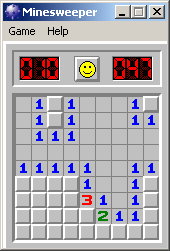
\includegraphics[scale=0.7]{\CURPATH/1.png}}
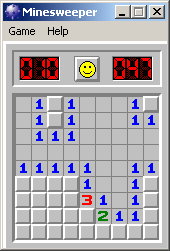
\includegraphics[scale=0.7]{\CURPATH/1.png}
\end{figure}

\subsubsection{Exercise}

... from the "Pearls in Graph Theory" book:

\begin{framed}
\begin{quotation}
1.1.1. Seven students go on vacations. They decide that each will send a postcard to three of the others.
Is it possible that every student receives postcards from precisely the three to whom he sent postcards?
\end{quotation}
\end{framed}

No, it's not possible, because 7*3 is a odd number.
However, if you reduce 7 students to 6, this is solvable, the sequence is [3,3,3,3,3,3].

Now the graph of mutual exchanging of postcards between 6 students:

\begin{figure}[H]
\centering
%\frame{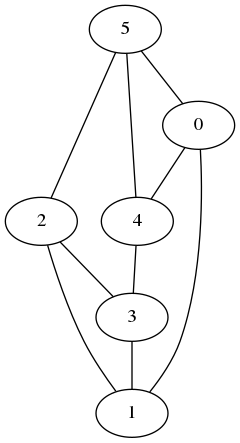
\includegraphics[scale=0.7]{\CURPATH/6_students.png}}
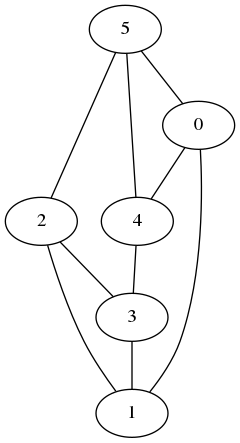
\includegraphics[scale=0.7]{\CURPATH/6_students.png}
\caption{6 students}
\end{figure}

